\documentclass[t]{beamer} %[t]
% dont use section page: sectionpage=none
\usetheme{metropolis}           % Use metropolis theme
\usepackage{appendixnumberbeamer}
\PassOptionsToPackage{table,svgnames,dvipsnames}{xcolor}

\usepackage[utf8]{inputenc}
\usepackage[T1]{fontenc}
\usepackage[sc]{mathpazo}
\usepackage[ngerman,english]{babel} % english is the same as american or USenglish
\usepackage[autostyle]{csquotes}
\usepackage[%
  backend=biber,
  url=true,
  style=numeric, % alphabetic, numeric
  sorting=none, % default == nty, https://tex.stackexchange.com/questions/51434/biblatex-citation-order
  %maxnames=4,
  maxcitenames=2,
  mincitenames=1,
  %minnames=3,
  maxbibnames=99,
  giveninits,
  uniquename=init]{biblatex} % TODO: adapt citation style
  %\ExecuteBibliographyOptions{maxcitenames=2,mincitenames=1}
\usepackage{graphicx}
%\usepackage{minted}
\usepackage{scrhack} % necessary for listings package
\usepackage{listings}
\usepackage{lstautogobble}
\usepackage{tikz}
\usepackage{pgfplots}
\usepackage{pgfplotstable}
\usepackage{booktabs} % for better looking table creations, but bad with vertical lines by design (package creator despises vertical lines)
\usepackage[final]{microtype}
\usepackage{caption}
%\usepackage[hidelinks]{hyperref} % hidelinks removes colored boxes around references and links
\usepackage{ifthen} % for comparison of the current language and changing of the thesis layout
\usepackage{pdftexcmds} % string compare to work with all engines
%\usepackage{paralist} % for condensed enumerations or lists
\usepackage{subfig} % for having figures side by side
\usepackage{siunitx} % for physical accurate units and other numerical presentations
\usepackage{multirow} % makes it possible to have bigger cells over multiple rows in a table
\usepackage{array} % different options for table cell orientation
\usepackage{makecell} % allows nice manual configuration of cells with linebreaks in \thead and \makecell with alignments
\usepackage{pdfpages} % for including multiple pages of pdfs
\usepackage{adjustbox} % can center content wider than the \textwidth
\usepackage{tablefootnote} % for footnotes in tables as \tablefootnote
\usepackage{threeparttable} % another way to add footnotes as \tablenotes with \item [x] <your footnote> after setting \tnote{x} 


% https://tex.stackexchange.com/questions/42619/x-mark-to-match-checkmark
\usepackage{amssymb}% http://ctan.org/pkg/amssymb
\usepackage{pifont}% http://ctan.org/pkg/pifont
\newcommand{\cmark}{\ding{51}}%
\newcommand{\xmark}{\ding{55}}%


% \usepackage[automake,acronym,xindy,toc]{glossaries} % TODO: include "acronym" if glossary and acronym should be separated
% \makeglossaries
% \loadglsentries{glossary.tex} % important update for glossaries, before document

% OWN PACKAGES
\usepackage{pgf-umlsd}
\usepgflibrary{arrows}
\usepackage[simplified]{pgf-umlcd}
%\usepackage{tikz-uml}
\usepackage{float}
\usepackage[fleqn,tbtags]{mathtools}
\usepackage{algorithm}
%\usepackage[noend]{algpseudocode}
%\usepackage[makeroom]{cancel}
\usepackage{algpseudocode}
\usepackage{glossary-longbooktabs}
\usepackage{hhline}
\usepackage[section]{placeins}
\usepackage{changes}
\usepackage{cancel}
\usepackage{soul}
%\definecolor{lightblue}{rgb}{.90,.95,1}
%\setstcolor{lightblue}

% --


\bibliography{bibliography}

%\setkomafont{disposition}{\normalfont\bfseries} % use serif font for headings
\linespread{1.05} % adjust line spread for mathpazo font

% Add table of contents to PDF bookmarks
\BeforeTOCHead[toc]{{\cleardoublepage\pdfbookmark[0]{\contentsname}{toc}}}

% Define TUM corporate design colors
% Taken from http://portajointl.mytum.de/corporatedesign/index_print/vorlagen/index_farben
\definecolor{TUMBlue}{HTML}{0065BD}
\definecolor{TUMSecondaryBlue}{HTML}{005293}
\definecolor{TUMSecondaryBlue2}{HTML}{003359}
\definecolor{TUMBlack}{HTML}{000000}
\definecolor{TUMWhite}{HTML}{FFFFFF}
\definecolor{TUMDarkGray}{HTML}{333333}
\definecolor{TUMGray}{HTML}{808080}
\definecolor{TUMLightGray}{HTML}{CCCCC6}
\definecolor{TUMAccentGray}{HTML}{DAD7CB}
\definecolor{TUMAccentOrange}{HTML}{E37222}
\definecolor{TUMAccentGreen}{HTML}{A2AD00}
\definecolor{TUMAccentLightBlue}{HTML}{98C6EA}
\definecolor{TUMAccentBlue}{HTML}{64A0C8}

% Settings for pgfplots
\pgfplotsset{compat=newest}
\pgfplotsset{
  % For available color names, see http://www.latextemplates.com/svgnames-colors
  cycle list={TUMBlue\\TUMAccentOrange\\TUMAccentGreen\\TUMSecondaryBlue2\\TUMDarkGray\\},
}

% Settings for lstlistings

% Use this for basic highlighting
\lstset{%
  basicstyle=\ttfamily,
  columns=fullflexible,
  autogobble,
  keywordstyle=\bfseries\color{TUMBlue},
  stringstyle=\color{TUMAccentGreen}
}

% use this for C# highlighting
% %\setmonofont{Consolas} %to be used with XeLaTeX or LuaLaTeX
% \definecolor{bluekeywords}{rgb}{0,0,1}
% \definecolor{greencomments}{rgb}{0,0.5,0}
% \definecolor{redstrings}{rgb}{0.64,0.08,0.08}
% \definecolor{xmlcomments}{rgb}{0.5,0.5,0.5}
% \definecolor{types}{rgb}{0.17,0.57,0.68}

% \lstset{language=[Sharp]C,
% captionpos=b,
% %numbers=left, % numbering
% %numberstyle=\tiny, % small row numbers
% frame=lines, % above and underneath of listings is a line
% showspaces=false,
% showtabs=false,
% breaklines=true,
% showstringspaces=false,
% breakatwhitespace=true,
% escapeinside={(*@}{@*)},
% commentstyle=\color{greencomments},
% morekeywords={partial, var, value, get, set},
% keywordstyle=\color{bluekeywords},
% stringstyle=\color{redstrings},
% basicstyle=\ttfamily\small,
% }
\definecolor{mygreen}{rgb}{0,0.6,0}
\definecolor{mygray}{rgb}{0.5,0.5,0.5}
\definecolor{mymauve}{rgb}{0.58,0,0.82}

\lstset{ 
  backgroundcolor=\color{white},   % choose the background color; you must add \usepackage{color} or \usepackage{xcolor}; should come as last argument
  %basicstyle=\footnotesize,        % the size of the fonts that are used for the code
  breakatwhitespace=false,         % sets if automatic breaks should only happen at whitespace
  breaklines=true,                 % sets automatic line breaking
  %captionpos=b,                    % sets the caption-position to bottom
  commentstyle=\color{mygreen},    % comment style
  %deletekeywords={...},            % if you want to delete keywords from the given language
  %escapeinside={\%*}{*)},          % if you want to add LaTeX within your code
  %extendedchars=true,              % lets you use non-ASCII characters; for 8-bits encodings only, does not work with UTF-8
  %firstnumber=1000,                % start line enumeration with line 1000
  %frame=single,	                   % adds a frame around the code
  keepspaces=true,                 % keeps spaces in text, useful for keeping indentation of code (possibly needs columns=flexible)
  keywordstyle=\color{blue},       % keyword style
  language=Python,                 % the language of the code
  %morekeywords={*,...},            % if you want to add more keywords to the set
  %numbers=left,                    % where to put the line-numbers; possible values are (none, left, right)
  numbersep=5pt,                   % how far the line-numbers are from the code
  numberstyle=\tiny\color{mygray}, % the style that is used for the line-numbers
  rulecolor=\color{black},         % if not set, the frame-color may be changed on line-breaks within not-black text (e.g. comments (green here))
  showspaces=false,                % show spaces everywhere adding particular underscores; it overrides 'showstringspaces'
  showstringspaces=false,          % underline spaces within strings only
  showtabs=false,                  % show tabs within strings adding particular underscores
  %stepnumber=2,                    % the step between two line-numbers. If it's 1, each line will be numbered
  stringstyle=\color{mymauve},     % string literal style
  %tabsize=2,	                   % sets default tabsize to 2 spaces
  %title=\lstname                   % show the filename of files included with \lstinputlisting; also try caption instead of title
}


% Settings for search order of pictures
\graphicspath{
    {logos/}
    {figures/}
}

% Set up hyphenation rules for the language package when mistakes happen
\babelhyphenation[english]{
an-oth-er
ex-am-ple
}

% Decide between
%\newcommand{\todo}[1]{\textbf{\textsc{\textcolor{TUMAccentOrange}{(TODO: #1)}}}} % for one paragraph, otherwise error!
%\newcommand{\done}[1]{\textit{\textsc{\textcolor{TUMAccentBlue}{(Done: #1)}}}} % for one paragraph, otherwise error!
% and
%\newcommand{\todo}[1]{{\bfseries{\scshape{\color{TUMAccentOrange}[(TODO: #1)]}}}} % for multiple paragraphs
%\newcommand{\done}[1]{{\itshape{\scshape{\color{TUMAccentBlue}[(Done: #1)]}}}} % for multiple paragraphs
% for error handling of intended behavior in your latex documents.

\newcommand{\tabitem}{~~\llap{\textbullet}~~}

\newcolumntype{P}[1]{>{\centering\arraybackslash}p{#1}} % for horizontal alignment with limited column width
\newcolumntype{M}[1]{>{\centering\arraybackslash}m{#1}} % for horizontal and vertical alignment with limited column width
\newcolumntype{L}[1]{>{\raggedright\arraybackslash}m{#1}} % for vertical alignment left with limited column width
\newcolumntype{R}[1]{>{\raggedleft\arraybackslash}m{#1}} % for vertical alignment right with limited column width

% OWN COMMANDS
\newcommand{\myceil}[1]{\left \lceil #1 \right \rceil }
\newcommand{\myfloor}[1]{\left \lfloor #1 \right \rfloor }
\newcommand{\norm}[1]{\left\lVert#1\right\rVert}

\newcommand{\kuka}{Kuka LBR iiwa}
\newcommand{\krl}{\texttt{keras-rl}}
\newcommand{\ke}{\texttt{keras}}
\newcommand{\myparagraph}[1]{\paragraph{#1}\mbox{}\\}
\newcommand{\dql}{Deep Q-Learning}
\newcommand{\ddpg}{Deep Deterministic Policy Gradient}
\renewcommand\textbullet{\ensuremath{\bullet}}


%\setlength{\parindent}{4em}
%\setlength{\parskip}{0.5em}

\AtBeginBibliography{\footnotesize}
\setbeamerfont{footnote}{size=\tiny}
\setbeamercolor{background canvas}{bg=white}
\citetrackerfalse

% \usepackage{tabularx}


% \usepackage[utf8]{inputenc}
% \usepackage[TS1,T1]{fontenc}
% \usepackage{array, booktabs}
% \usepackage{graphicx}
% \usepackage{caption}
% \usepackage{animate}


% \setbeamerfont{footnote}{size=\tiny}
% \setbeamercolor{background canvas}{bg=white}


\title{Validation Tool for \texttt{libmoeprlnc}}
% \date{\today}
\date{April 22, 2022}
\author{Group 6\\Tobias Jülg and Ben Riegel}
% \subtitle{Course 7, Ferienakademie 2021}
\institute[TUM]{Technical University of Munich}
\setbeamertemplate{footline}[frame number]
\setbeamertemplate{bibliography item}[text]

% \setbeamertemplate{frame footer}{\insertshortauthor~(\insertshortinstitute)}
% \setbeamerfont{page number in head/foot}{size=\tiny}
% \setbeamercolor{footline}{fg=gray}


\begin{document}
\maketitle

%\metroset{sectionpage=none}

\section{Introduction}
\begin{frame}{Why should \texttt{libmoeprlnc} need validation?}
  \begin{columns}
  \column{.5\textwidth}
  % TODO: Example image
    \begin{figure}[htb]
      \centering
      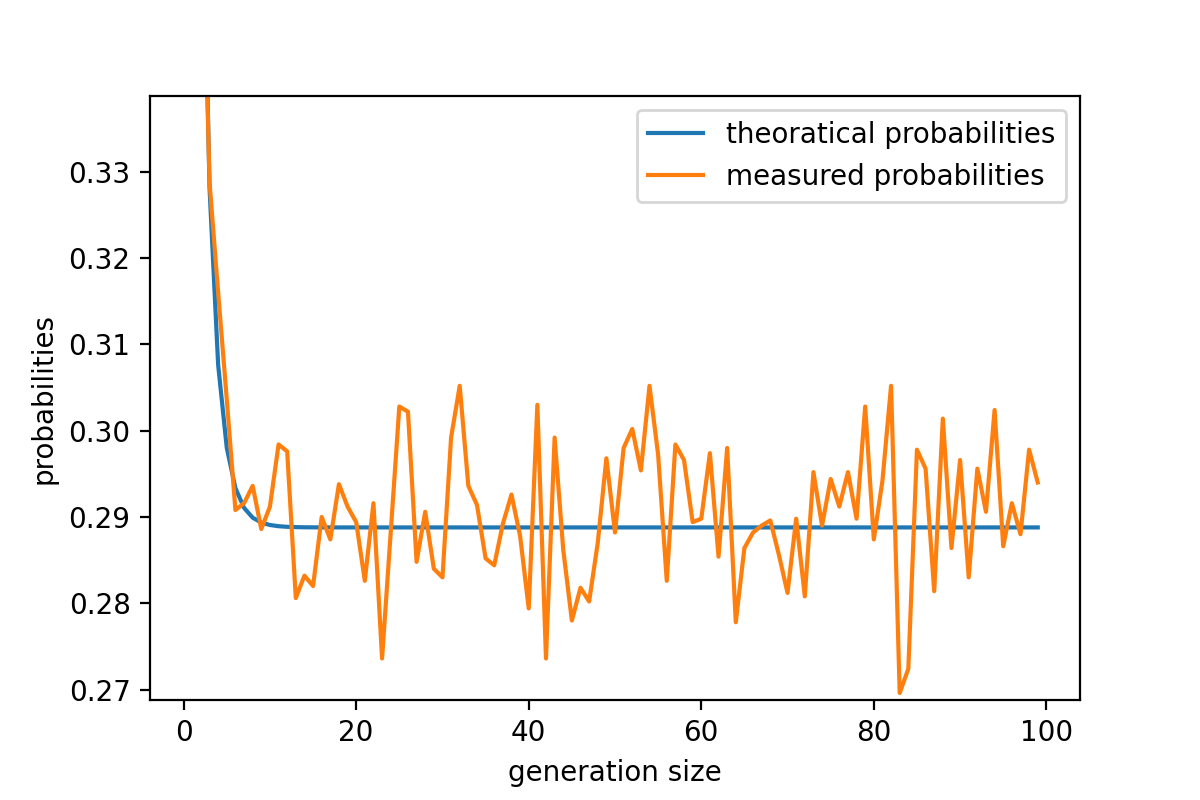
\includegraphics[scale=0.16]{figures/gf2}
    \end{figure}
  \column{.5\textwidth}
  \begin{itemize}
    \item ...
  \end{itemize}
  \end{columns}
\end{frame}

\begin{frame}{Outline}
  \setbeamertemplate{section in toc}[sections numbered]
  \tableofcontents %[hideallsubsections]
\end{frame}


% Methodology
\section{Idea and Methodology}
\begin{frame}{Basic Idea}
  % \vspace{-0.3cm}
    \begin{figure}[htb]
      % \centering
  % \hspace{-1cm}
  \begin{tikzpicture}
    \node[draw] at (0, 2)   (ga) {Generation A};
    \node[draw] at (0, 0)   (ba) {\texttt{rlnc\_block} A};
    \node[draw] at (6, 2)   (gb) {Generation B};
    \node[draw] at (6, 0)   (bb) {\texttt{rlnc\_block} B};
    \draw [thick,->] (ga) -- (ba) node[midway,left] {\texttt{create\_at\_A()}};
    \draw [thick,->] (ba) -- (bb) node[midway,below] {\texttt{transmit\_A2B()}};
    \draw [thick,->] (bb) -- (gb) node[midway,right] {\texttt{consume\_at\_B()}};
  \end{tikzpicture}
    \end{figure}
  % \footnotesize
  \pause
  \begin{itemize}
    % todo mention random drop
    % \item Two participants A and B with unidirectional traffic
    \visible<7>{\item repeat for $n$ iterations}
    \begin{itemize}
    \item Create random generation at A
  \pause
    \item \texttt{create\_at\_A} adds the next uncoded frame to \texttt{rlnc\_block} at A
  \pause
    \item \texttt{transmit\_A2B} creates a RLC frame from A, drops it with specified prob. and puts it into the \texttt{rlnc\_block} at B
  \pause
    \item \texttt{consume\_at\_B} tires to read the next unencoded frame from B
  \pause
    \item Compare unencoded generation from B with the one at A
    \end{itemize}
  \end{itemize}
\end{frame}

\begin{frame}{Modes}
  \textbf{Random Mode}
  \begin{itemize}
    \item Random order of \texttt{create\_at\_A}, \texttt{transmit\_A2B} and \texttt{consume\_at\_B}
    \item Used to find rare bugs in \texttt{libmoeprlnc} as execution order that haven't been thought of are also tested
    \item e.g. trying to encode and sent a frame when no frames have been added to the generation on A
    \pause
    \item[$\rightarrow$] Problematic for statistical evaluation
  \end{itemize}
  \pause
  \textbf{Prefill Mode}
  \begin{itemize}
    \item First add all frames to A, then encode and transmit all frames and finally decode them at B
    \item Used for statistical evaluation
  \end{itemize}
\end{frame}

\section{Results and Evaluation}

\begin{frame}{Overall Outcome}
  \begin{itemize}
    \item In the end, all of our tests both modes run through without problems
    \item Statistical validation agrees to theoretical expectations
    \item We discovered two minor things
  \end{itemize}
\end{frame}


\begin{frame}{Linear Independency: Theory}
  Probability of $N$ frames being linear independent for generation size $N$ no matter the frames size, where $q$ is the Galois Field size:%\\
  % probability that N randomly linear coded frames are sufficient for transmitting with generation size $N$
\begin{equation} 
  \text{Pr}\left[\text{dim}\bigcup_{i=1}^{N}\{c_i\} = N\right] = \prod_{i=1}^{N} \left(1 - \frac{q^{i - 1}}{q ^ {N}}\right)
  \label{eq:decode_prob}
\end{equation}
\begin{itemize}
  \item[$\rightarrow$] Prob. that $N$ randomly linear coded transmitted frames are sufficient for decoding
% To verify the correspondence the theoratical prob
  \item[$\rightarrow$] Have to use prefill mode
  \item For each supported\footnote{$q\in\{2, 4, 16, 256\}$} $q$ we run our validation for increasing\footnote{$N\in[100]$} $N$
  \item For each $N$ we transmitted 5000 frames and counted the ones that finished after $N$ transmission
  % \item[$\righarrow$] Prob. of succ. trans. after $N$ for 
  % counted the over 5000 iterations to the prob.
\end{itemize}
\end{frame}

\begin{frame}{Linear Independency: Measurements I}
  \vspace{-1cm}
\begin{figure}
  \centering
  \subfloat[$q=2$]{  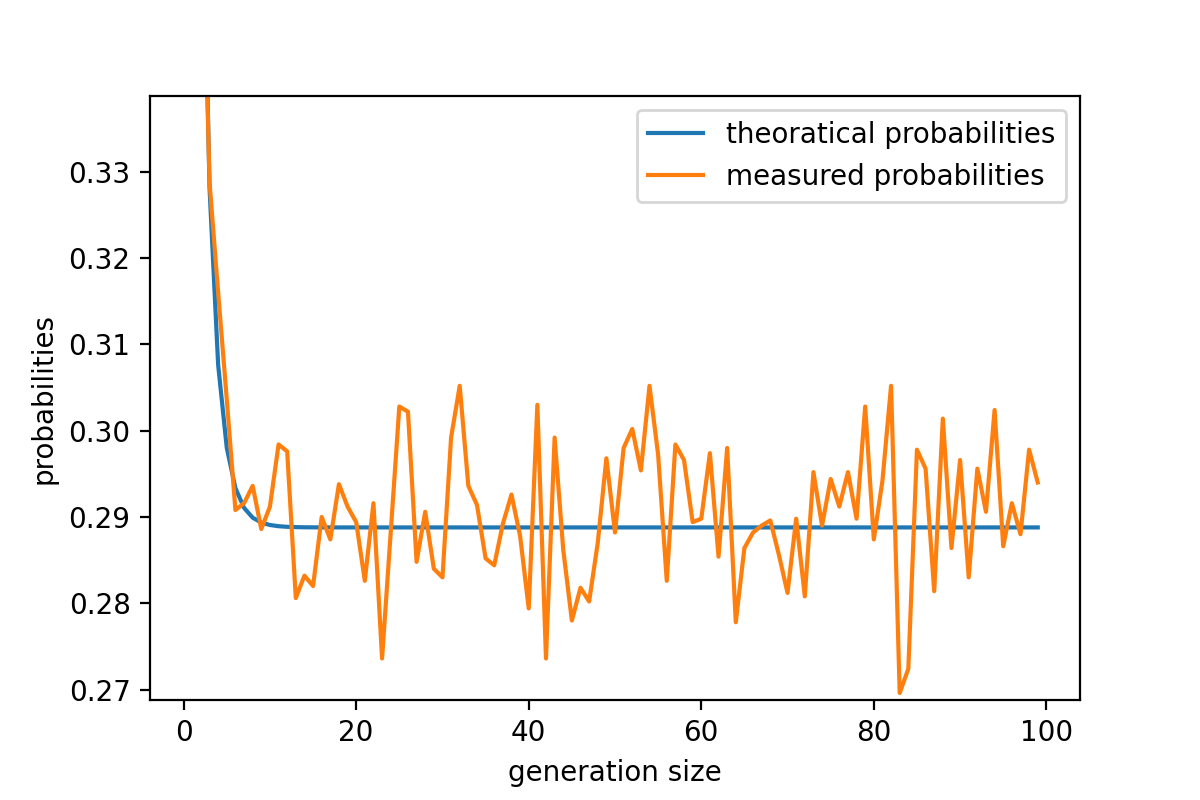
\includegraphics[scale=0.33]{figures/gf2}\label{fig:gf2}}
  \hfill
  \subfloat[$q=4$]{  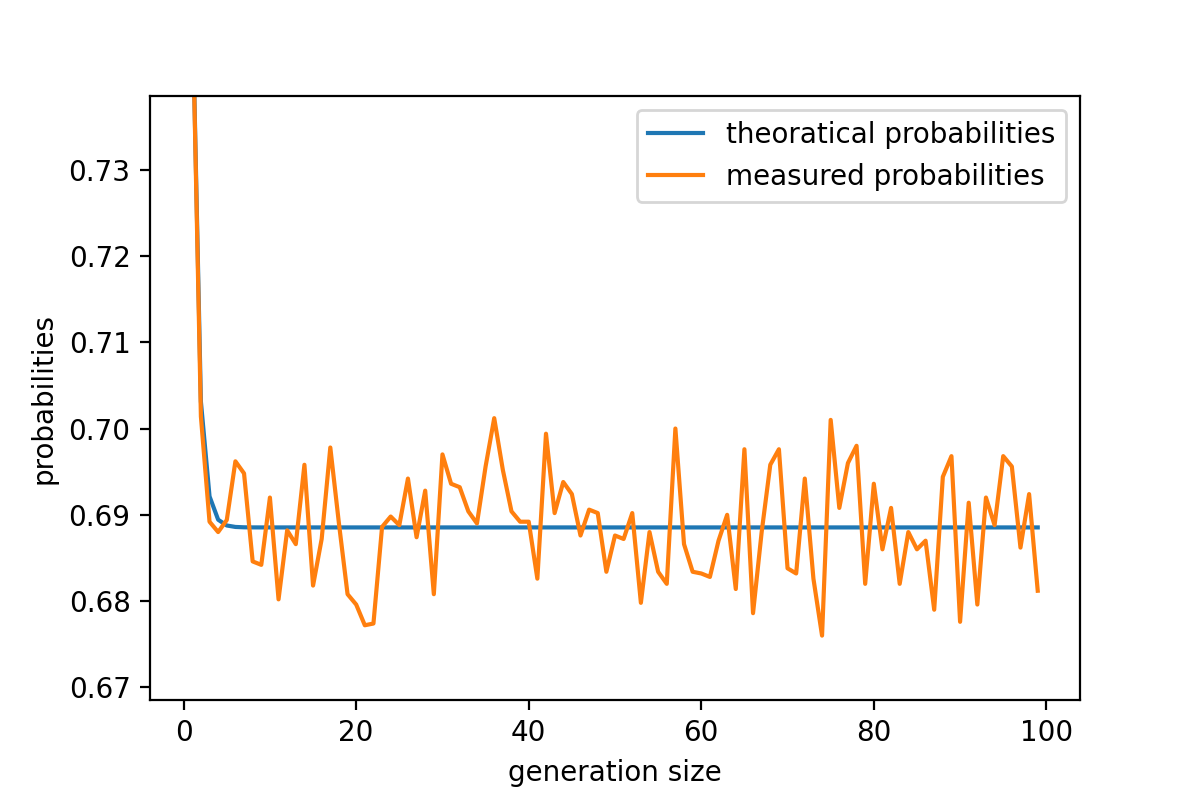
\includegraphics[scale=0.33]{figures/gf4}\label{fig:gf4}}
  \hfill
  \subfloat[$q=16$]{ 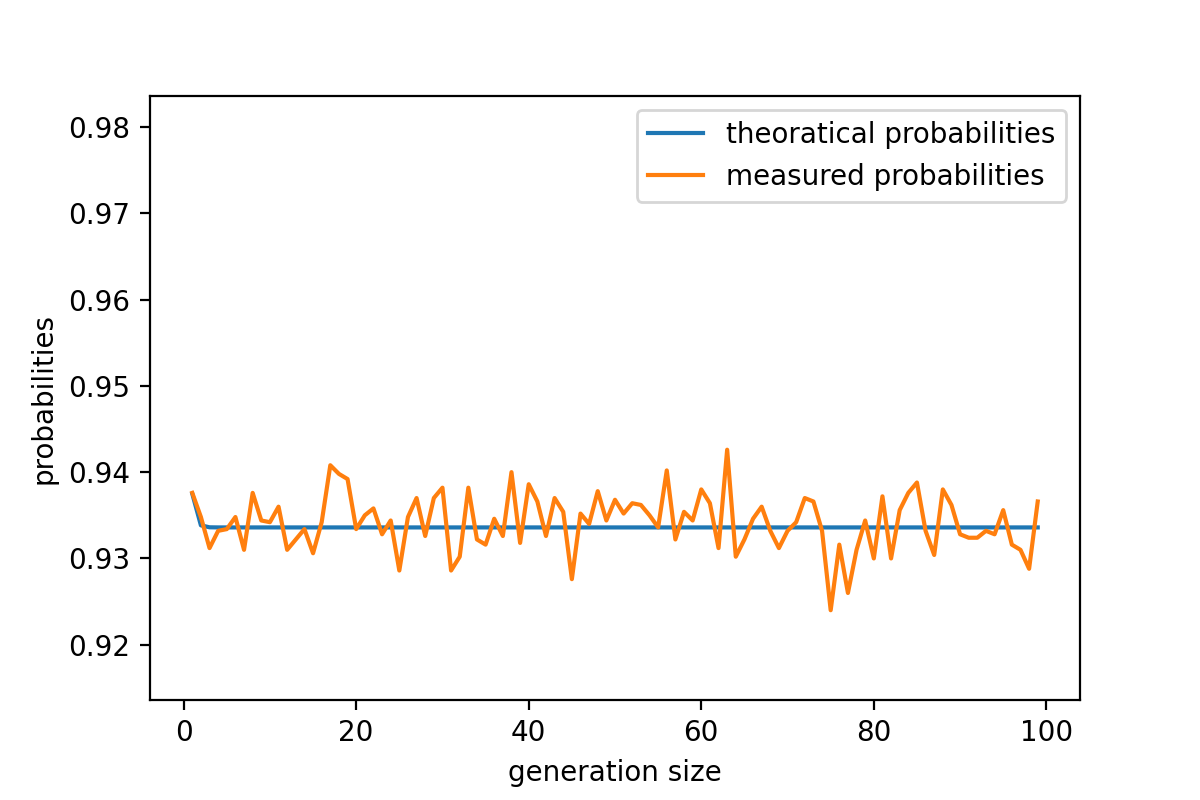
\includegraphics[scale=0.33]{figures/gf16}\label{fig:gf16}}
  \hfill
  \subfloat[$q=256$]{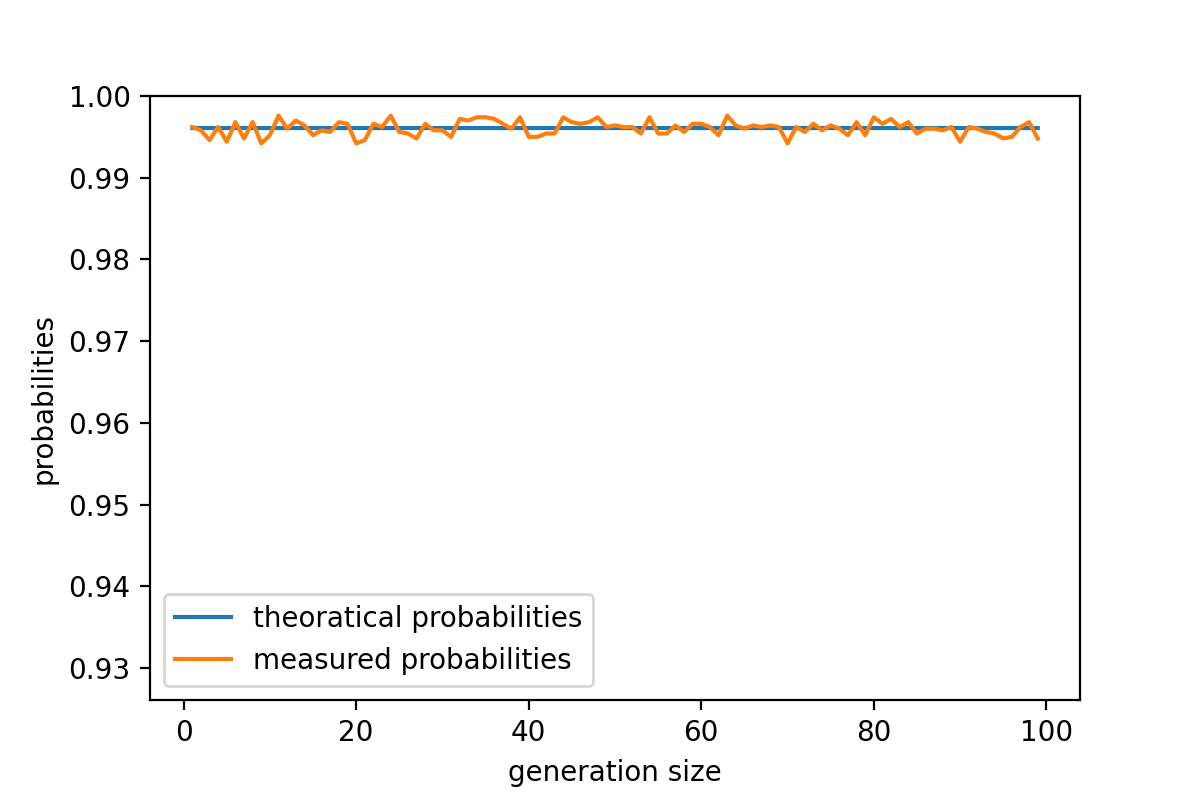
\includegraphics[scale=0.33]{figures/gf256}\label{fig:gf256}}
  %\caption{...}\label{fig:gfs}
\end{figure}
\end{frame}

\begin{frame}{Linear Independency: Measurements II}
\begin{table}[htb]
  \caption{Mean, standard deviation and theoretical lower bound for the plots over $N\ge20$ in percentage}
  \label{tab:mean-std}
  \centering
  \begin{tabular}{l|l|l|l}
    \toprule
       $q$ & Mean & Standard Deviation & Lower Bound \\
    \midrule
    2 & 29.04\% & $\pm$0.81\% & 28.88\%\\
    4 & 68.87\% & $\pm$0.62\% & 68.85\%\\
    16 & 93.41\% & $\pm$0.33\% & 93.36\%\\
    256 & 99.61\% & $\pm$0.08\% & 99.61\%\\
    \bottomrule
  \end{tabular}
\end{table}
\end{frame}

\begin{frame}{What we discovered}
  \begin{itemize}
    \item Missing check in \texttt{$rlnc\_block\_decode$} whether the passed length corresponds to the expected size
    \item Seed always set to zero and not changeable by the user
    \item[$\rightarrow$] Leads always to same coding vectors if everything else unchanged
    \item[$\rightarrow$] Extreme results, bad for statistical evaluation
  \end{itemize}
    \begin{figure}[htb]
      \centering
      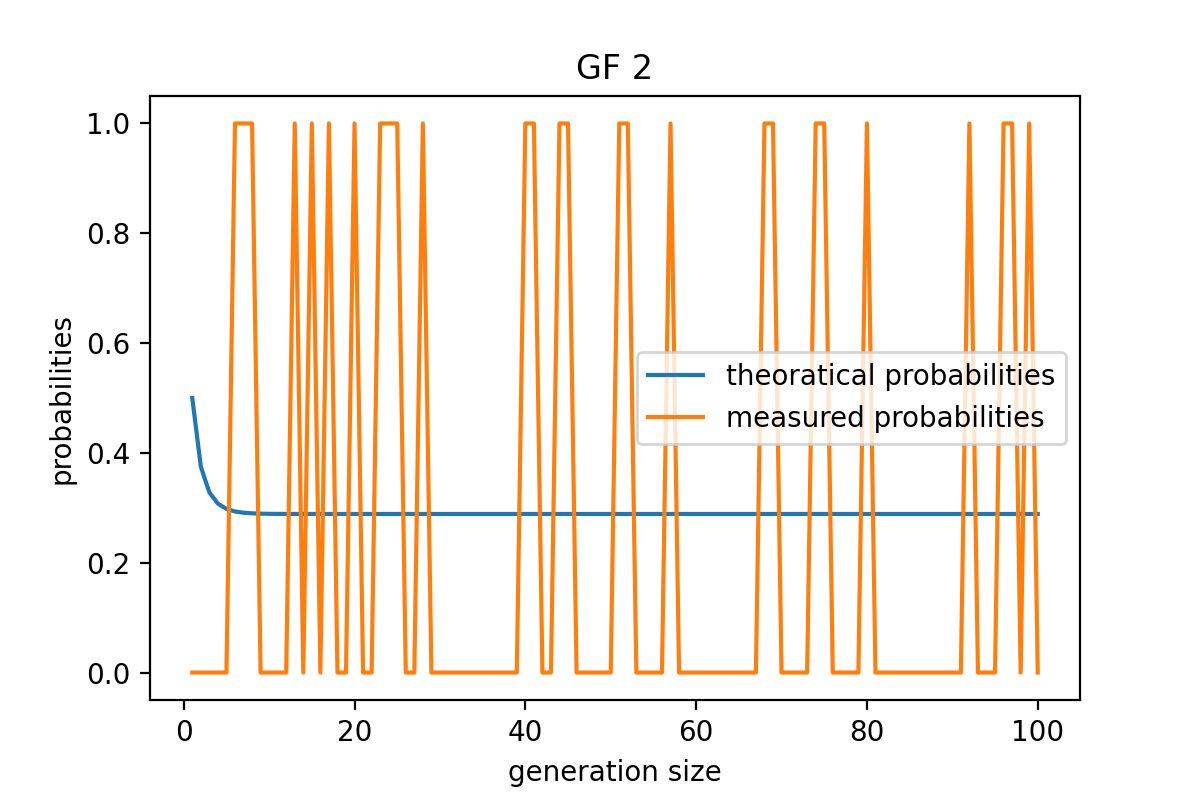
\includegraphics[scale=0.45]{figures/gf2_noseed}
    \end{figure}
\end{frame}




% often hard to use as badly documented, often guess and find out with debugging or read the code, this is not how an api should work :(
% build system poluted, why is there no build folder, would make your git life much easier...
\begin{frame}[standout]
  Live Demo!
\end{frame}

% if we have references:
% \metroset{sectionpage=none}
% \begin{frame}[allowframebreaks]{References}
%   % \nocite{...}
%   \footnotesize
%   \printbibliography{}
% \end{frame}

% Backup slides go here
\appendix
\metroset{sectionpage=simple}
\section{Backup}
\begin{frame}{...}
  \begin{itemize}
    \item ...
  \end{itemize}
\end{frame}


\end{document} 
